\chapter{Evolution of system design}
\label{chap:evolution}

To track sleep unobtrusively, multiple techniques and sensor types have been tested and evaluated by other researchers. Piezoelectric film sensor were placed on a rodent cage and signals were used for recognition of breathing and movement\cite{piezo}. In same way, sleep and awakening was recorded in humans using load cells placed under bed supports\cite{load_cells}. Subjects were also recorded using infrared cameras and this method provided 19\% better recognition of small movements than actigraphy done with a wrist worn device\cite{video}. \ac{POF} sensors were also used to recognize breathing patterns and detect apnea\cite{optical}. In another research, a group of researchers conducted experiment in which they placed two 24\ac{GHz} radars under the bed in a nursing home and found out that it is possible to accurately recognize the hearth rate\cite{radar}. Using pressure sensitive e-textile it is possible to classify a sleep stage as awake, \ac{NREM} or \ac{REM}\cite{e-textile}. And using pneumatic pressure sensors placed in a sealed air-cushion that is placed under the bed it is possible to measure hearth beat, respiration, snoring and movement\cite{pneumatic}. The work of Prof. Dr. Ralf Seepold, Ra\'ina Kuhn, Daniel Scherz and Maxime Guyot at \ac{UC-Lab}\cite{Kuhn}\cite{Guyot} on which this thesis continues is using pressure sensors to determine position, detect movement and track vital signs.

\section{Devices and technology}

There are multiple types of pressure sensors that could be used for the purpose of this project\cite{pressure_sensors}. Potentiometric pressure sensors are very crude due to their construction and often have realiability and hysteresis problems. Inductive pressure sensors require \ac{AC} excitation of coils and therefore demodulation and filtering needs to be done to get a result. Piezoelectric and piezoresistive pressure sensors measure change of pressure by using piezoelectric effect. Capacitive pressure sensors use a small diaphragm as a capacitor plate. When pressure is applied, diaphragm deflects and capacitance changes. Change may or may not be linear and usually is on the order of a few \ac{pF} while total capacitance of the sensor is between 50 and 100 \ac{pF}. This method suffers from environmental effects and may be influenced by \ac{PCB} or protoboard\footnote{A standardized electronics prototyping board which usually features a grid of electrically connected holes.} design. \ac{FSR} is a type of material whose resistance changes when a force is applied. Since this material can have a larger surface, it can be used as a pressure sensor. Advantages of \ac{FSR} sensors over other pressure sensor is its accuracy, possibility of detecting a static pressure, flexibility, thinness and inexpensiveness. Multiple other researches were made used the same type of sensor and have proven its reliability and accuracy when used in a sensor mesh\cite{pillow_system_1}\cite{pillow_system_2}\cite{apnea_low_cost}. Therefore it is a type of sensor that was selected for this specific project.

So how does the \ac{FSR} sensor work? \ac{FSR} is a \ac{PTF} device which exhibits a decrease in resistance with an increase in the force applied to the active surface\cite{fsr_guide}. At 'zero force' state conductive ink is separated from the active area by spacer adhesive and in that case \ac{FSR} sensor has highest possible resistance. When pressure is applied to sensor, conductive layer is pushed down on active area which results in a decrease of resistance. Construction of FSR sensor is provided in \ref{fig:fsr-sensor}. For a hemispherical sensor with diameter of 12.7mm (type \#402) sensibility starts just below 20g and extends to 10kg when saturation occurs. Passing a threshold, or 'break force', changes resistance from greater than 100 $k\Omega$ to 10 $k\Omega$. After that resistance falls logarithmically with the increase of force as seen in \ref{fig:fsr-sensor}. What application manual\cite{fsr_guide} suggests using a firm, flat and smooth mounting surface and using of a rubber spring to spread the pressure over whole sensor.

\begin{figure}[h]
  \begin{center}
    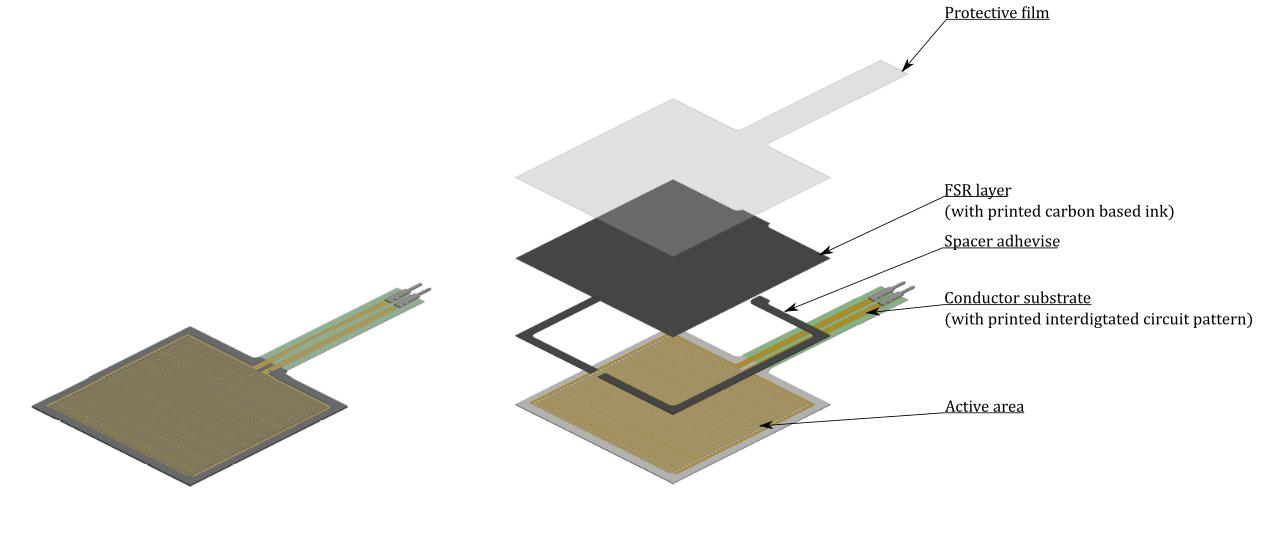
\includegraphics[width=0.58\linewidth]{1-fsr_sensor.png}
    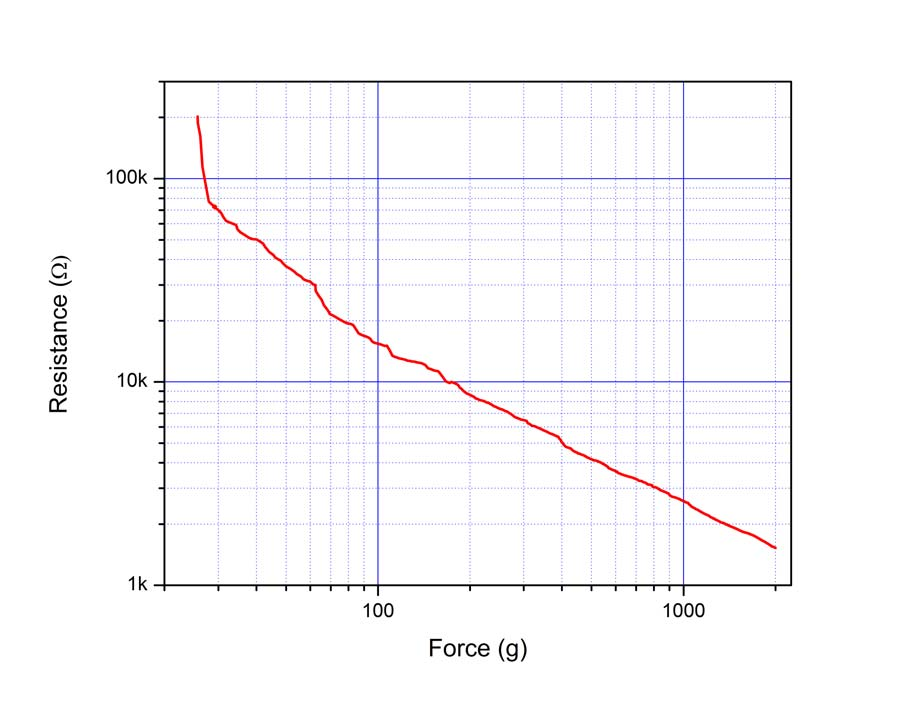
\includegraphics[width=0.35\linewidth]{1-fsr_graph.png}
  \end{center}
  \caption{FSR sensor construction and resistance characteristics.}
  \label{fig:fsr-sensor}
\end{figure}

\begin{figure}[h]
  \begin{center}
    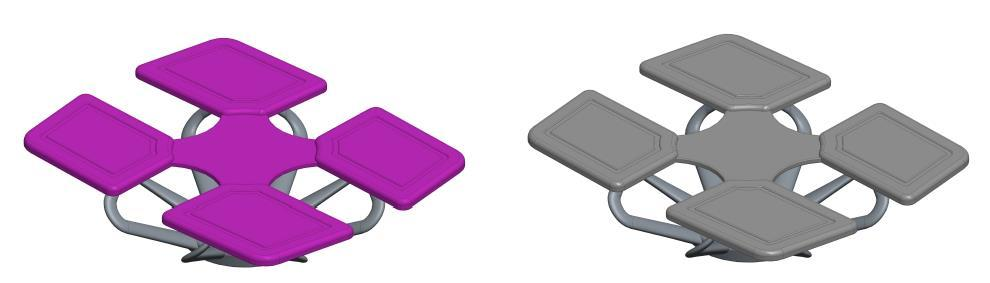
\includegraphics[width=0.6\linewidth]{1-base_plate.jpg}
  \end{center}
  \caption{Base plates in the bed.}
  \label{fig:base-plate}
\end{figure}


\section{Test environment}

\begin{figure}[h]
  \begin{center}
    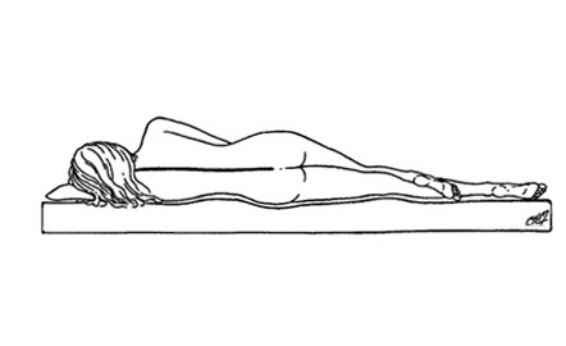
\includegraphics[width=0.4\linewidth]{1-weight_distribution.png}
    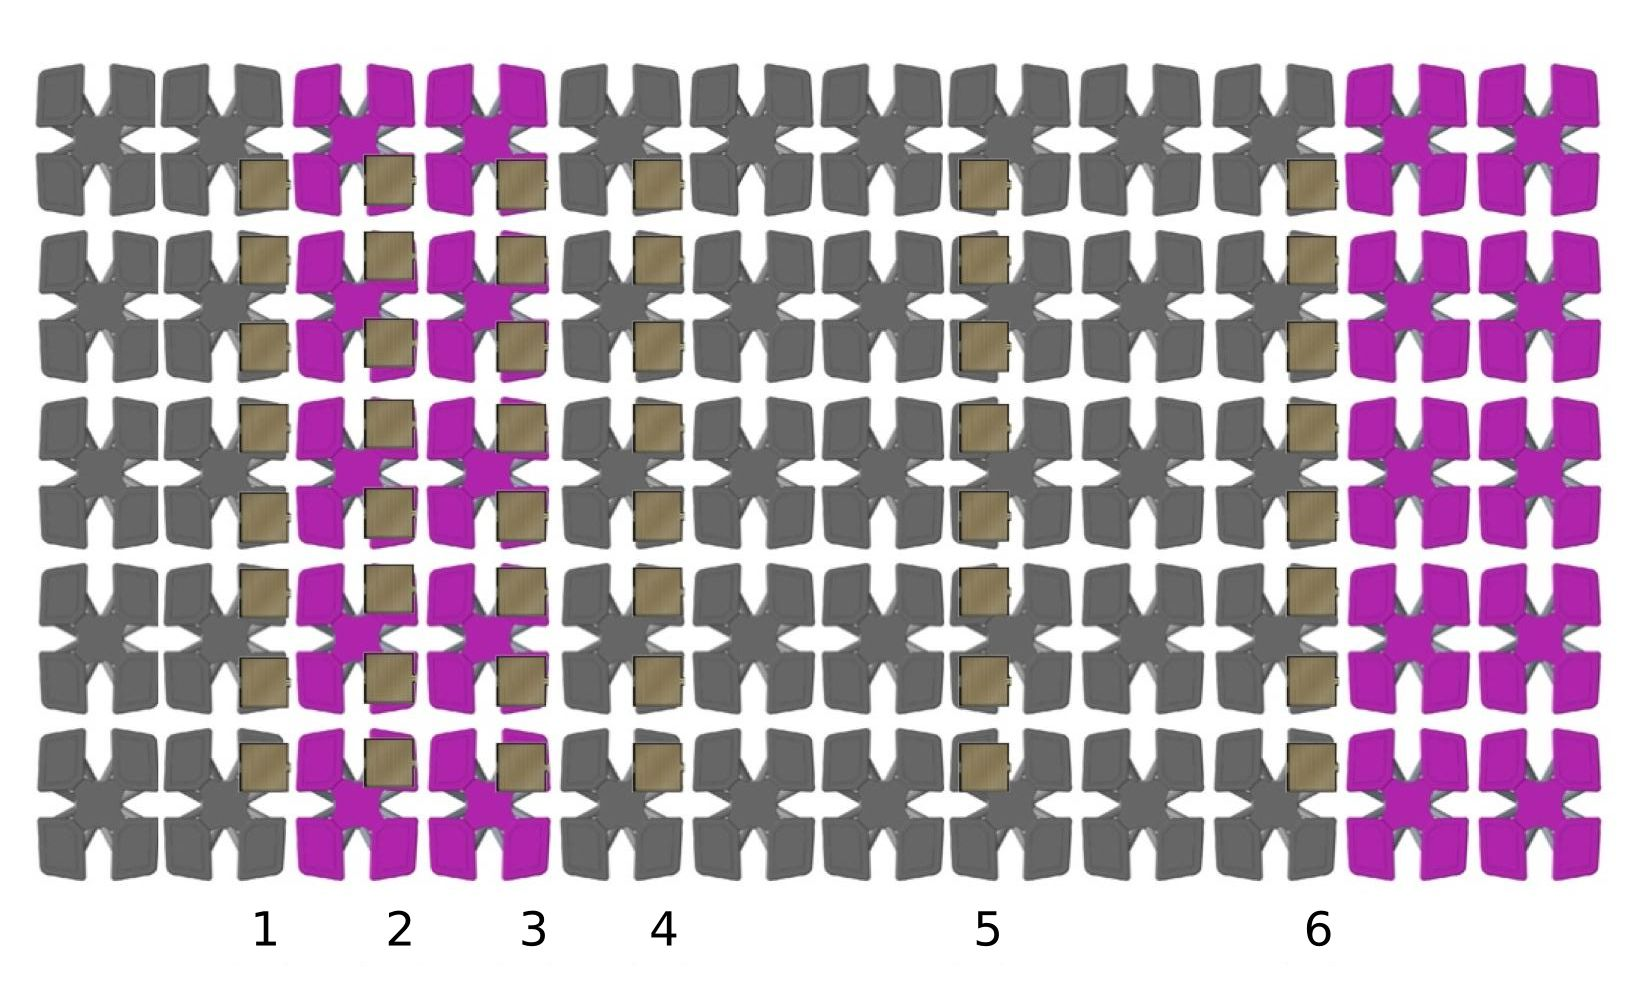
\includegraphics[width=0.4\linewidth]{1-sensor_layout.jpg}
  \end{center}
  \caption{Sensor arrangement in bed compared to sleep position.}
  \label{fig:sensor-layout}
\end{figure}

\begin{figure}[h]
  \begin{center}
    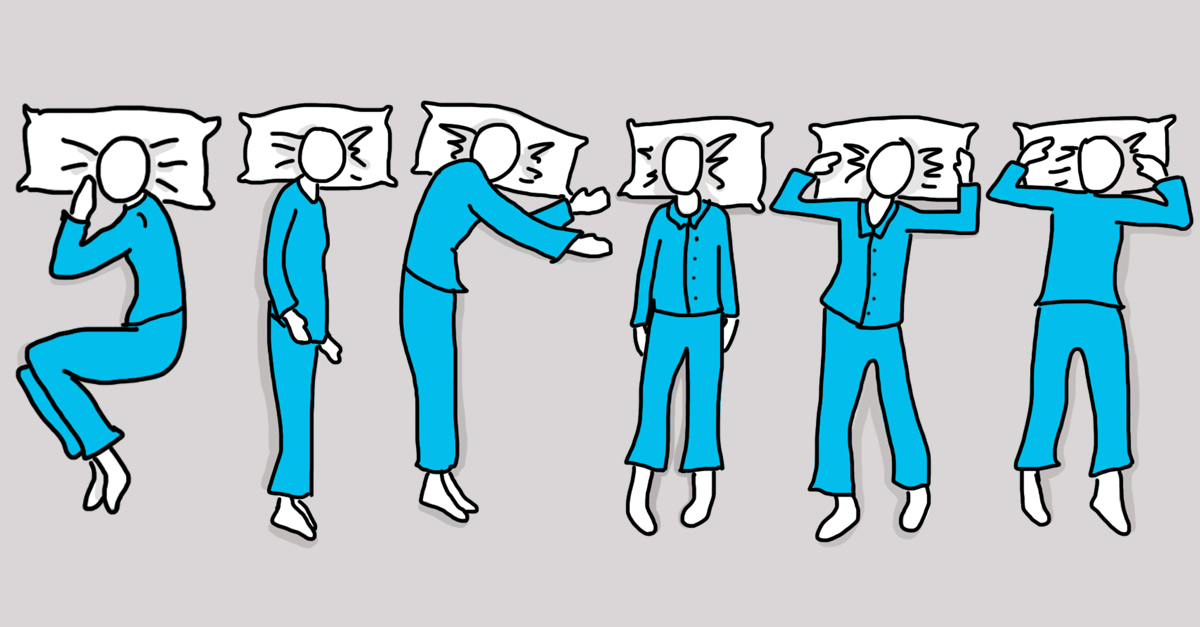
\includegraphics[width=0.4\linewidth]{1-sleep_positions.jpg}
  \end{center}
  \caption{Different sleep positions.}
  \label{fig:sleep_positions}
\end{figure}


\section{Results so far}


